%! TEX root = pertemuan_kebutuhan_ruang.tex
% the main TeX file which is intended to compile, :VimtexReload after adjustment
   % this file should be included in the main file
% :h vimtex-tex-root
\documentclass[../spa_2.tex]{subfiles}
%ensure the class of docs

\begin{document}

\bglightimg{kebutuhan_ruang}

\bglightimg{program_ruang_1}
\bglightimg{program_ruang_2}
\bglightimg{program_ruang_3}
\bglightimg{program_ruang_4}
\bglightimg{program_ruang_5}

\begin{frame}[mytitle=standard,t,mycolor=digiPH_white,light]
	\frametitle{Kebutuhan Ruang}
	\begin{center}
		Tugas
	\end{center}
	\txt{digiPH_ocean}{digiPH_white}{\begin{itemize}
			\item Analisis Pelaku Kegiatan
			\item   Analisis Kebutuhan dan Besaran Ruang
		\end{itemize}}
\end{frame}

\bglightimg{organisasi_11}
\begin{frame}[mytitle=standard,c,mybg=bglight3,light]
	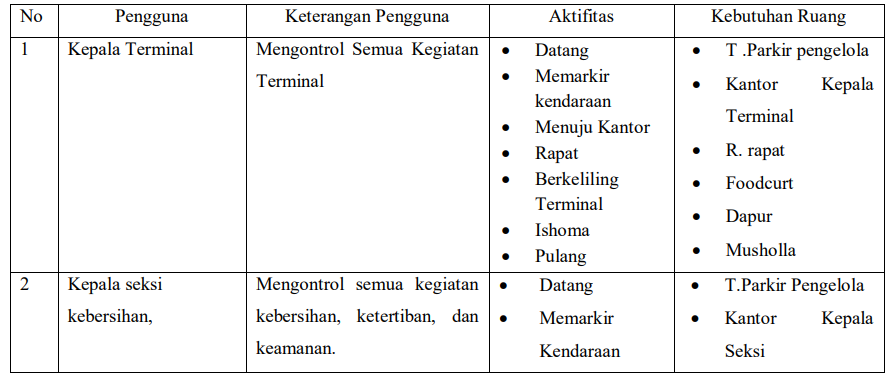
\includegraphics[width=.92\textwidth]{../figures/pelaku_1}
\end{frame}

\bglightimg{program_ruang_6}
\bglightimg{program_ruang_7}

\bibliographystyle{apalike}
\bibliography{../filename.bib} % required for citecompletion, not work in mainfile
\end{document}

